\documentclass[authoryear,11pt]{elsarticle}

%This eliminates the `Preprint submitted to...' footer on the first page
\makeatletter
\def\ps@pprintTitle{%
 \let\@oddhead\@empty
 \let\@evenhead\@empty
 \def\@oddfoot{}%
 \let\@evenfoot\@oddfoot}
\makeatother

\usepackage{amssymb}
\usepackage{amsthm}
\usepackage{caption}
\usepackage{amsmath}
\usepackage{morefloats}
\usepackage{bbm}        %To allow \mathbb{1}

\usepackage{rotating}   %To turn tables sidewaystable
\usepackage{graphicx}
\usepackage{setspace}
\usepackage{hyperref}

%\onehalfspacing

%\setlength{\parindent}{0pt}

\usepackage[top=3.5cm,bottom=3.75cm,left=2.45cm,right=2.45cm]{geometry}% by courtesy of Mico

\begin{document}
\begin{frontmatter}
\title{MFE Economics\\Problem set 1}
\end{frontmatter}

%%%%%%%%%%%%%%%%%%%%%%%%%%%%%%%%%%%%%%%%%%%%%%%%%%%%%%%%%%%%%%%%%%%%%%%%%%%%%%%%%%%%%%%%%%%%%%%%%%%%%%%%%%%%%%%%%%%%%%%%%%%%%%%%%%%%%%%%%%%%%%%%%%%%%%%%
%%%%%%%%%%%%%%%%%%%%%%%%%%%%%%%%%%%%%%%%%%%%%%%%%%%%%%%%%%%%%%%%%%%%%%%%%%%%%%%%%%%%%%%%%%%%%%%%%%%%%%%%%%%%%%%%%%%%%%%%%%%%%%%%%%%%%%%%%%%%%%%%%%%%%%%%

\section{Problems based on lecture}

\subsection{Trends etc.}
\begin{figure}[!h]
\caption[Fed Funds Rate and Inflation]{Fed Funds Rate and Inflation - Trends and Cycles}
\centering
\label{fig:macro_series}
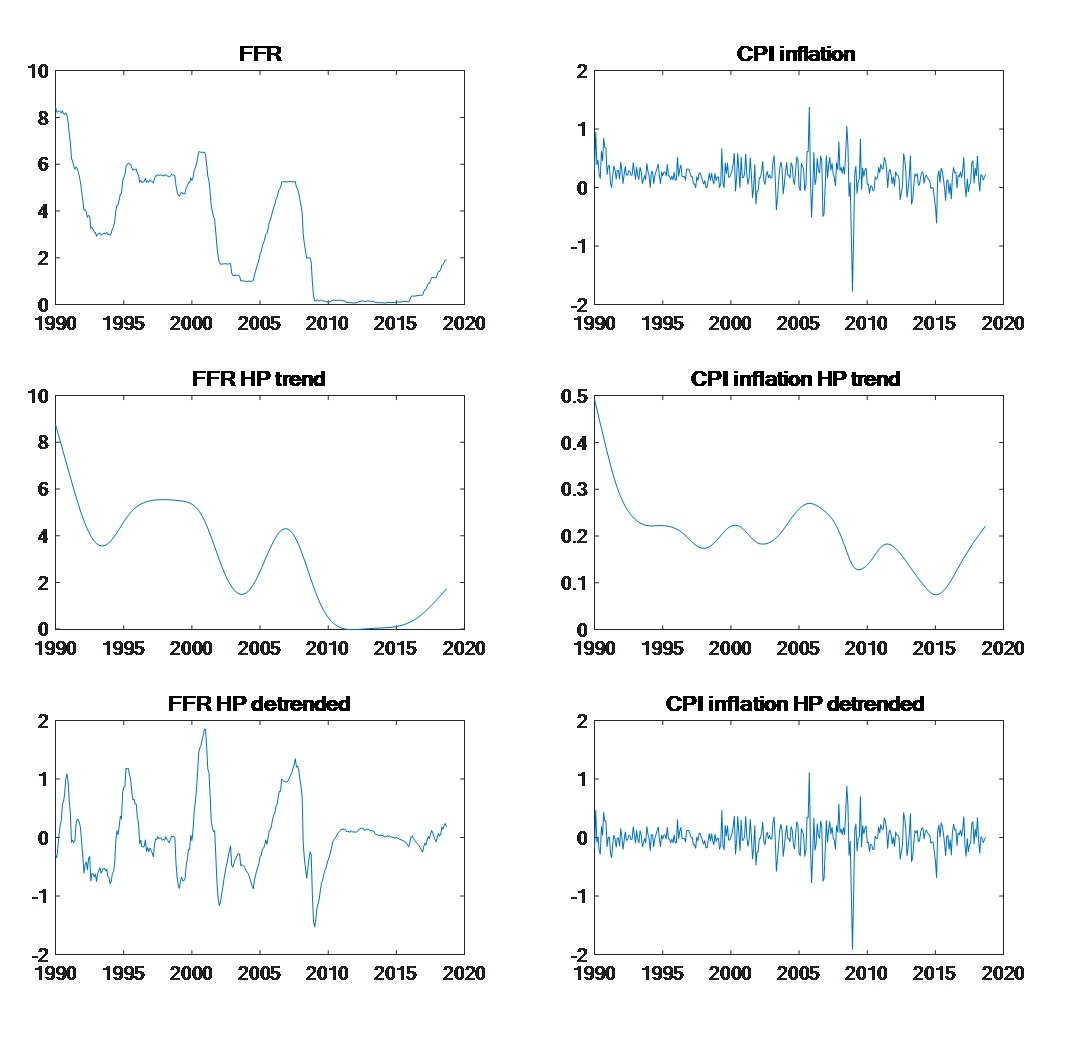
\includegraphics[width=0.55\textwidth]{macro_series.JPG}
\end{figure}

The first row in figure \ref{fig:macro_series} shows monthly data for the Federal Funds Rate and CPI inflation for the period 1990m1-2018m8. The remaining rows show the Hodrick-Prescott trend and cycle (with smoothing parameter $\lambda =14400$, the standard value for monthly data). Comment on the trends identified in the data and what they imply for the detrended data in the third row of the figure.

%\subsubsection*{Trends etc. - Answers}
%There is a clear downward trend in interest rates but not in inflation. This means that detrending matters for interest rates but not so much for inflation. Some would argue that the fall in interest rates is caused by other factors (demographics and secular stagnation) so removing the trend is valid.

\subsection{Structural VARS (SVARS)}
We are interested in the effects of interest rate (monetary policy) shocks on inflation. To begin, we estimate an unrestricted bivariate VAR with 4 lags in $R_{t}$ (HP detrended) and $\pi _{t}$ (demeaned but not detrended).

\begin{eqnarray*}
\left( 
\begin{array}{c}
R_{t} \\ 
\pi _{t}
\end{array}
\right) &=&\left( 
\begin{array}{cc}
1.32 & -0.02 \\ 
0.31 & 0.45
\end{array}
\right) \left( 
\begin{array}{c}
R_{t-1} \\ 
\pi _{t-1}
\end{array}
\right) \\
&&+\left( 
\begin{array}{cc}
-0.25 & 0.03 \\ 
-0.23 & -0.18
\end{array}
\right) \left( 
\begin{array}{c}
R_{t-2} \\ 
\pi _{t-2}
\end{array}
\right) \\
&&+\left( 
\begin{array}{cc}
-0.02 & -0.02 \\ 
-0.29 & 0.02
\end{array}
\right) \left( 
\begin{array}{c}
R_{t-3} \\ 
\pi _{t-3}
\end{array}
\right) \\
&&+\left( 
\begin{array}{cc}
-0.10 & -0.07 \\ 
0.26 & 0.03
\end{array}
\right) \left( 
\begin{array}{c}
R_{t-4} \\ 
\pi _{t-4}
\end{array}
\right) \\
&&+\left( 
\begin{array}{c}
u_{1t} \\ 
u_{2t}
\end{array}
\right) \\
&& \\
&&\text{with} \\
&& \\
\left( 
\begin{array}{c}
u_{1t} \\ 
u_{2t}
\end{array}
\right) &\sim &N\left[ \left( 
\begin{array}{c}
0 \\ 
0
\end{array}
\right) ;\left( 
\begin{array}{cc}
0.0147 & 0.0057 \\ 
0.0057 & 0.0511
\end{array}
\right) \right]
\end{eqnarray*}
Assume that interest rates react to shocks to inflation with a lag (this could be justified if the central bank does not have access to the current inflation data when it decides on policy, the Bernanke-Blinder (1992) identification), in which case the residuals of the bivariate VAR are related to the `structural' disturbances by
\[
\left( 
\begin{array}{c}
u_{1t} \\ 
u_{2t}
\end{array}
\right) =\left( 
\begin{array}{cc}
\theta _{1} & 0 \\ 
\theta _{3} & \theta _{4}
\end{array}
\right) \left( 
\begin{array}{c}
e_{1t} \\ 
e_{2t}
\end{array}
\right) 
\]

Calculate the coefficients $\theta_{1},\theta_{3},\theta_{4}$ implied by the estimation. Note that we assume that the structural shocks are uncorrelated with eachother and `standard normal' (mean 0 and unity variance):
\begin{equation*}
\left( 
\begin{array}{c}
e_{1t} \\ 
e_{2t}
\end{array}
\right) \sim N\left[ \left( 
\begin{array}{c}
0 \\ 
0
\end{array}
\right) ;\left( 
\begin{array}{cc}
1 & 0 \\ 
0 & 1
\end{array}
\right) \right]
\end{equation*}

Note also that if a vector $x$ has covariance matrix $\Sigma$ then the vector $Kx$ where $K$ is a matrix, will have covariance matrix, $K \Sigma K'$.

%\subsubsection*{Answers}
%We have $\sigma _{1}=\theta_{1}^{2}=0.0147,\sigma _{12}=\theta _{1}\theta _{3}=0.0057,\sigma_{2}=\theta _{3}^{2}+\theta _{4}^{2}=0.0511$. It follows that
%\[
%\left( 
%\begin{array}{cc}
%\theta _{1} & \theta _{2} \\ 
%\theta _{3} & \theta _{4}
%\end{array}
%\right) =\left( 
%\begin{array}{cc}
%0.1212 & 0 \\ 
%0.0469 & 0.2211
%\end{array}
%\right) 
%\]

\subsection{Responses to shocks}
The Excel spreadsheet MFE\_week3\_class.xlsx (available from the course webpage) is already part-programmed to help you produce impulse response functions from the estimate parameters of the VAR and different identification schemes.

Use the spreadsheet to calculate the impulse response functions to interest rate shocks and inflation shocks, under the assumption that shocks
to inflation do not affect the interest rate within the period. To do this you simply need to transfer the values of $\theta _{1},\theta _{3},\theta_{4}$ you just calculated into cells C3, C4, D3 and D4 of the spreadsheet (hint, D3 will be zero when inflation shocks do not contemporaneously affect interest rates). The spreadsheet checks whether your values of $\theta _{1},\theta _{3},\theta _{4}$ are consistent with the variance-covariance matrix of residuals of the VAR in cells A13 and A14 (i.e. have you done your calculation correctly). If they are then you should see some sensible impulse responses. What is the response of the economy to an interest rate shock? And to an inflation shock? Do these make intuitive sense? If not, what might be wrong?
%
%\subsubsection*{Answers}
%The interest rate shock increases inflation, which is counterintuitive and we have a price puzzle. In addition, interest rates barely react to inflation shocks, if anything falling slightly. This is again counterintuitive as we would expect monetary policy to raise the interest rate after an inflation shock.
%
%\begin{figure}[!h]
%\caption[Response to interest rate shock]{Response to interest rate shock}
%\centering
%\label{fig:macro_series}
%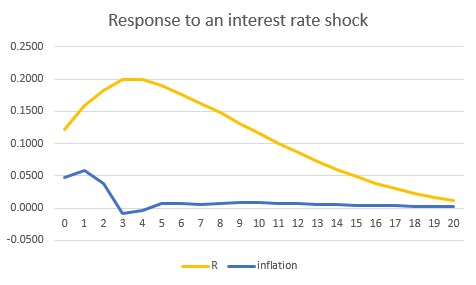
\includegraphics[width=0.55\textwidth]{response_to_irate.JPG}
%\end{figure}
%
%\begin{figure}[!h]
%\caption[Response to inflation shock]{Response to inflation shock}
%\centering
%\label{fig:macro_series}
%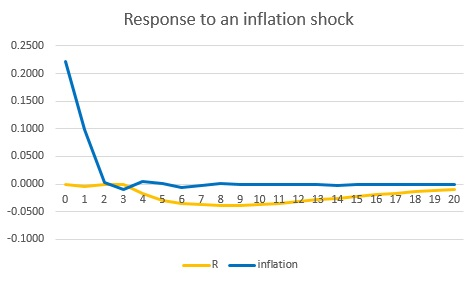
\includegraphics[width=0.55\textwidth]{response_to_inflation.JPG}
%\end{figure}

\section{Math Problems}

\subsection{Linearizations and log-linearizations - basic examples}
In the appendix of the lecture 1 slides there is a discussion of linearizations and log-linearizations that you should read before attempting questions in this section. I assume that you are comfortable with simple calculus (basic differentiation) and the use of logarithms (logs) and exponential functions, though there is a refresher of some of their most relevant properties in the note on the webpage.

\begin{itemize}
\item	Linearize $5 + 3x^{2}$ around $\bar{x}$. Now linearize it around $x=1$ and $x=2$ (i.e. set $\bar{x}=1$ and $\bar{x}=2$). Roughly sketch a picture of the exact function and the approximating functions in the vicinity of the two specified approximation points. What is the value of the exact function and approximated functions at $x=1$, $x=2$ and $x=3$? Comment on the approximation errors.
\item	Log linearize $15 - 3xy^2$ around $(\bar{x},\bar{y})$. Now log-linearize it around $(x,y)=(2,3)$. What is the value of the exact function at $(1,4)$ and what is the value of the approximating function.
\end{itemize}

%\subsubsection*{Answers}
%We have that $f'(x) = 6x$ so the linearization is
%\begin{eqnarray*}
%f(x) 	&\approx& f(\bar{x}) + f'(\bar{x})(x-\bar{x})	\\
%	&=& 5+3\bar{x}^2+6\bar{x}(x-\bar{x})		\\
%	&=& \psi_{0} + \psi_{1}x
%\end{eqnarray*}
%where $\psi_{0}\equiv5-3\bar{x}^2$ and $\psi_{1}\equiv 6\bar{x}$. Since the approximation depends on the $\bar{x}$ chosen we can make this explicit by writing the approximating function as
%\[
%\hat{f}(x;\bar{x}) = \psi_{0}(\bar{x}) + \psi_{1}(\bar{x}) x
%\]
%
%If we take $\bar{x}$ to be $1$ and $2$ in turn, we have (see figure \ref{fig:lin_diagram} for sketches)
%\begin{eqnarray*}
%\hat{f}(x;1) &=& 2 + 6x \\
%\hat{f}(x;2) &=& -7 + 12x 
%\end{eqnarray*}
%
%\begin{figure}[!htb]
%\center{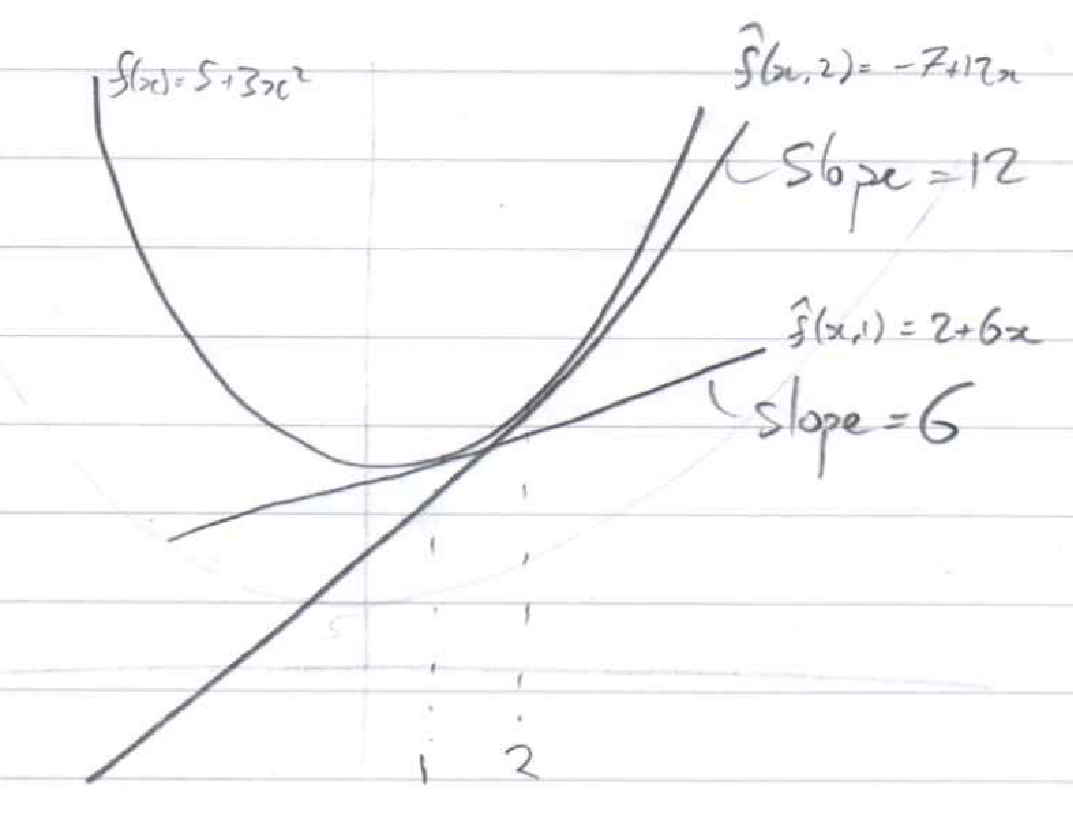
\includegraphics[width=0.6\textwidth]{lin_diagram.pdf}}
%\caption{\label{fig:lin_diagram} Sketch of exact and approximating functions}
%\end{figure}
%
%Table \ref{tab:approx_error} shows that the choice of approximation point ($\bar{x}$) can affect the quality of approximation at various evaluation points ($x$). In \emph{this} case we see that the closer we are to the approximation point, the smaller the errors.\footnote{This doesn't hold for \emph{arbitrary} points in the more general case (with more general functions, say) but the basic idea that the approximation point matters is what I am trying to convey.} In practice, the selection of an approximation point is very important as many economic models require some sort of approximation for us to be able to solve them. If the type of approximation used is as discussed in class (a `local' solution method such as linearizing or using higher order Taylor approximations) then the selection of the approximation point will typically depend on the problem at hand.
%
%\begin{table}[!htb]
%\centering
%\begin{tabular}{ c | c | c | c | c | c}
%\textbf{x} 	& $\mathbf{f(x)}$ 	& $\mathbf{\hat{f}_{1}(x)}$ 	& \textbf{Error} 	& $\mathbf{\hat{f}_{2}(x)}$ 	& \textbf{Error}	\\ \hline \hline
%  1			& $8$				& $8$						& $0$			& $5$						& $-3$			\\
%  2			& $17$				& $14$						& $-3$			& $17$						& $0$			\\
%  3			& $32$				& $20$						& $-12$			& $29$						& $-3$			\\ \hline \hline
%\end{tabular}
%\caption{Approximation quality and dependence on approximation point, $\bar{x}$}
%\label{tab:approx_error}
%\end{table}
%
%Imagine a situation (outside the scope of our course) where maybe we are interested in approximating an agent's consumption function, where consumption depends on asset holdings, $a_{t}$. In this case we would be approximating $c_{t} = f(a_{t})$ around some $\bar{a}$ for some complicated function, $f$. The model may imply that, over time, $a_{t}$ evolves randomly but spends `most of its time' somewhat near its average value $E[a_{t}]$ and only occasionally drops to extremely low levels, say, in the vicinity of $a_{low}<<E[a_{t}]$. Assuming we want our approximation to perform well `most of the time' we would likely want to choose an approximation point near the average value, rather than near $a_{low}$, whereas if we are particularly concerned with behavior at low wealth levels, we might actually set $\bar{a}=a_{low}$.
%
%Now let us consider the second example, where $f(X,Y) = 15 - 3 XY^{2}$. In this case we are required to do a log-linearization which, as discussed in the notes, can be obtained by re-expressing in terms of log versions of the variables and then doing a linearization in terms of these transformed variables. Thus, we define a function $g$ such that $g(x,y) \equiv f(X,Y)$ (for $x\equiv \log{(X)}$ and $y\equiv \log{(Y)}$ and then linearize $g$. We have that
%\begin{eqnarray*}
%g(x,y)		&\equiv& 15 - 3e^{x+2y}	\\
%g_{x}(x,y)	&=& -3e^{x+2y}			\\
%y_{y}(x,y)	&=& -6e^{x+2y}
%\end{eqnarray*}
%
%The approximation is then given by
%\begin{eqnarray*}
%f(X,Y) 	&\equiv& 	g(x,y) \approx g(\bar{x}, \bar{y}) + g_{x}(\bar{x},\bar{y})(x-\bar{x}) + g_{y}(\bar{x},\bar{y})(y-\bar{y}) \\
%		&=&		15 - 3e^{\bar{x}+2\bar{y}}  -3e^{\bar{x}+2\bar{y}}(x-\bar{x}) - 6e^{\bar{x}+2\bar{y}}(y-\bar{y})
%\end{eqnarray*}
%
%If we take the approximation point for $f$ to be $(\bar{X},\bar{Y})=(2,3)$ then the approximation point for $g$ is $(\bar{x},\bar{y})=(\log{(2)},\log{(3)})$ and we obtain
%\[
%\hat{g}(x,y) \approx 117.08 -54 x - 108 y
%\]
%which implies that at $(X,Y)=(1,4)$ (equivalently $(x,y)=(0,\log{(4)})$) we have the exact value of the function of $-33$ whereas the approximating value is $-32.64$.

\subsection{Linearizations and log-linearizations - economics/financial example}
Campbell and Shiller (1988) propose a very useful approximation to the return on an asset that enables the price of that asset to be expressed in terms of its future stream of returns and dividends. For a more extensive analysis (on which this is based) see the notes on Simon Gilchrist's website.

The realized return on an asset from $t$ to $t+1$ is given by
\[
R_{t+1} \equiv \frac{P_{t+1} + D_{t+1}}{P_{t}}
\]
where $P_{t}$ is \emph{ex dividend} price of the asset in $t$ and, $D_{t}$ is the dividend paid in $t$. The return is made up of any dividend payment next period, plus the value of holding the asset next period, relative to the price paid today (i.e. capital gains). If we take logs of both sides we can express log returns as follows (you should understand these steps)
\begin{eqnarray}
\log{(R_{t+1})} 	&\equiv& \log{(P_{t+1} + D_{t+1})} - \log{(P_{t})}		\nonumber		\\
				&\equiv& \log{(P_{t+1}(1 + \frac{D_{t+1}}{P_{t+1}}))} - \log{(P_{t})}\nonumber \\
				&\equiv& p_{t+1} - p_{t} + \log{(1+ \exp{(d_{t+1} - p_{t+1})})} \label{eqn:log_ret}
\end{eqnarray}
Note that at this point we have not yet taken any approximations but, as I mention in the notes, it has been setup in a way that is amenable to doing a linearization in the (lower case $p_{t}\equiv\log{(P_{t})}$ etc.) log forms of the variables, which is equivalent to a log-linearization in terms of the original versions of the variables.

\begin{itemize}
\item Linearize $\log{(1+ \exp{(d_{t+1} - p_{t+1})})}$ around $(\bar{p},\bar{d})$ and show that\footnote{Really you just need to show $\log{(1+ \exp{(d_{t+1} - p_{t+1})})} 	\approx 	\log{(1+e^{d-p})} +\frac{e^{d-p}}{1+e^{d-p}}(d_{t+1}-d) - \frac{e^{d-p}}{1+e^{d-p}}(p_{t+1}-p)$ and then try and rearrange terms appropriately. In fact, we should really be doing this linearization in terms of the (log) dividend-price ratio, $dp_{t+1}\equiv d_{t} - p_{t+1}$ as there may be no natural constant steady state value of dividends or prices, due to growth (and/or inflation, if these are expressed in nominal terms) but let us ignore that for now.}
\[
\log{(1+ \exp{(d_{t+1} - p_{t+1})})} 	\approx 	k + (1-\rho)(d_{t+1}-p_{t+1}) \\
\]
where
\begin{eqnarray*}
\rho		&\equiv&	(1+\exp{(\bar{d}-\bar{p})})^{-1} \\
k		&\equiv&	-\log{(\rho)} - (1-\rho)\log{(\rho^{-1} - 1)}
\end{eqnarray*}

\item Use the above approximation, along with equation (\ref{eqn:log_ret}), to obtain
\[
p_{t} = \rho p_{t+1} + k + (1-\rho)d_{t+1} - r_{t+1}
\]
and, therefore,
\[
p_{t}-d_{t} = \rho (p_{t+1}-d_{t+1}) + k + \Delta d_{t+1} - r_{t+1}
\]

\item Denoting $\delta_{t} \equiv p_{t}-d_{t}$, show that this implies (hint: keep substituting for $\delta_{t+1}$, $\delta_{t+2}$,\ldots on the RHS)
\begin{equation}
\delta_{t} = \frac{k}{1-\rho} + \sum\limits_{j=0}^{\infty} \rho^{j}(\Delta d_{t+1+j} - r_{t+1+j}) \label{eqn:expost}
\end{equation}
\end{itemize}

Though you don't need to know this for the course, what is useful about this relation is that (with error only arising from the linear approximation) it shows that variation in the price dividend ratio must be accompanied by variations in future dividend growth, or future returns, or both. This holds \emph{ex post} (subject only to approximation error from the linearization) but, in addition, the relationship holds \emph{ex ante}. That is, one can take expectations of each side to say (note that $E_{t}[p_{t} - d_{t}] = p_{t}-d_{t}$ as the price-dividend ratio in $t$ is known at $t$):
\[
\delta_{t} = \frac{k}{1-\rho} + \sum\limits_{j=0}^{\infty} \rho^{j}E_{t}[\Delta d_{t+1+j} - r_{t+1+j}]
\]

%\subsubsection*{Answers}
%Let $f(p_{t+1},d_{t+1}) \equiv \log{(1+e^{d_{t+1}-p_{t+1}})}$ then we have
%\begin{eqnarray*}
%f_{p}(p_{t+1},d_{t+1}) &=& - \frac{e^{d_{t+1}-p_{t+1}}}{1+e^{d_{t+1}-p_{t+1}}}	\\
%f_{d}(p_{t+1},d_{t+1}) &=& \frac{e^{d_{t+1}-p_{t+1}}}{1+e^{d_{t+1}-p_{t+1}}}
%\end{eqnarray*}
%and we can construct a first order approximation as (let's just use $p$ and $d$ instead of $\bar{p}$ and $\bar{d}$ here)
%\begin{eqnarray}
%f_{d}(p_{t+1},d_{t+1}) 	&\approx& 	f(p,d) + f_{p}(p,d)(p_{t+1}-p) + f_{d}(p,d)(d_{t+1}-d)	\nonumber \\
%						&=&		\log{(1+e^{d-p})}- \frac{e^{d-p}}{1+e^{d-p}} (p_{t+1}-p) + \frac{e^{d-p}}{1+e^{d-p}} (d_{t+1}-d)	\label{eqn:step_1}\\
%						&=&		-\log{(\rho)} - \frac{e^{d-p}}{1+e^{d-p}} (d-p) + \frac{e^{d-p}}{1+e^{d-p}} (d_{t+1}-p_{t+1}) \label{eqn:step_2}
%\end{eqnarray}
%where in going from equation (\ref{eqn:step_1}) to equation (\ref{eqn:step_2}) we used the definition of $\rho$. Now, we note that
%\[
%1-\rho \equiv 1 - \frac{1}{1+e^{d-p}} = \frac{e^{d-p}}{1+e^{d-p}}
%\]
%so we can rewrite equation (\ref{eqn:step_2}) as
%\begin{equation}
%f_{d}(p_{t+1},d_{t+1}) = -\log{(\rho)} - (1-\rho)(d-p) + (1-\rho)(d_{t+1}-p_{t+1}) \label{eqn:step_3}
%\end{equation}
%Further, we note that
%\[
%\rho^{-1} - 1 = 1+e^{d-p}-1 = e^{d-p}
%\]
%which implies $\log{(\rho^{-1} - 1)}=d-p$. Using this in equation (\ref{eqn:step_3}) we obtain the desired expression.
%
%We then have
%\[
%r_{t+1} \approx p_{t+1} - p_{t} + k + (1-\rho)(d_{t+1} - p_{t+1})
%\]
%Or, rearranging (and dropping the $\approx$ symbol)\ldots
%\begin{eqnarray*}
%p_{t} 	&=& p_{t+1} + k + (1-\rho)(d_{t+1} - p_{t+1}) - r_{t+1} \\
%		&=& \rho p_{t+1} + k + (1-\rho)d_{t+1} - r_{t+1}
%\end{eqnarray*}
%Then, subtracting $d_{t}$ from each side (and using the notation $\Delta Z_{t} \equiv Z_{t} - Z_{t-1}$) we have
%\begin{equation}
%p_{t}-d_{t} = \rho (p_{t+1}-d_{t+1}) + k + \Delta d_{t+1} - r_{t+1} \label{eqn:step_4}
%\end{equation}
%
%Finally, letting $\delta_{t} \equiv p_{t} - d_{t}$ equation (\ref{eqn:step_4}) implies
%\begin{eqnarray*}
%\delta_{t} 	&=& 	\rho \delta_{t+1} + k + \Delta d_{t+1} - r_{t+1}	\\
%			&=&	\rho (\rho \delta_{t+2} + k + \Delta d_{t+2} - r_{t+2}) + k + \Delta d_{t+1} - r_{t+1} \\
%			&=&	\rho (\rho (\rho \delta_{t+3} + k + \Delta d_{t+3} - r_{t+3}) + k + \Delta d_{t+2} - r_{t+2}) + k + \Delta d_{t+1} - r_{t+1} \\
%			&=&	k \sum\limits_{j=0}^{J} \rho^{j} + \sum\limits_{j=0}^{J} \rho^{j}( \Delta d_{t+1+j} - r_{t+1+j} ) + \rho^{J+1} \delta_{t+1+J}
%\end{eqnarray*}
%Then if we let $J\to \infty$ and assume (a `transversality condition') $\rho^{J+1} \delta_{t+1+J} \to 0$ then we obtain the desired result (noting that $ \sum\limits_{j=0}^{\infty} \rho^{j} = \frac{1}{1-\rho}$)
%\[
%\delta_{t} = \frac{k}{1-\rho} + \sum\limits_{j=0}^{\infty} \rho^{j}(\Delta d_{t+1+j} - r_{t+1+j})
%\]

\end{document}

